\section{Neural Networks}
In the field of machine learning, statistical algorithms are commonly employed for data analysis. 
Neural networks, a specific category of such algorithms, have experienced exponential growth in 
usage in both industry and academia over the past decade. These models find extensive use in a 
variety of applications, ranging from image analysis to weather prediction. The fundamental principle 
behind feed forward neural networks (FFNN) involves the data being fed forward through the network,
 with the end output evaluated and corrections then back propagated through the network to update 
 the weights and biases. This training process is repeated until a certain threshold is met. 
 figure \ref{fig:nndiagram} depicts a general layout of a neural network, wherein the input layer consists of 
 one node per feature in the dataset. The number of hidden layers and nodes per layer can be 
 fine-tuned, with the last hidden layer connected to the output layer. The latter is determined 
 by the problem being addressed, and in the case of the binary classification problem depicted 
 in figure \ref{fig:nndiagram}, the nodes interact via tunable weights $w$ and biases $b$ that must 
 be trained on the dataset prior to making predictions.

\begin{figure}[H]
    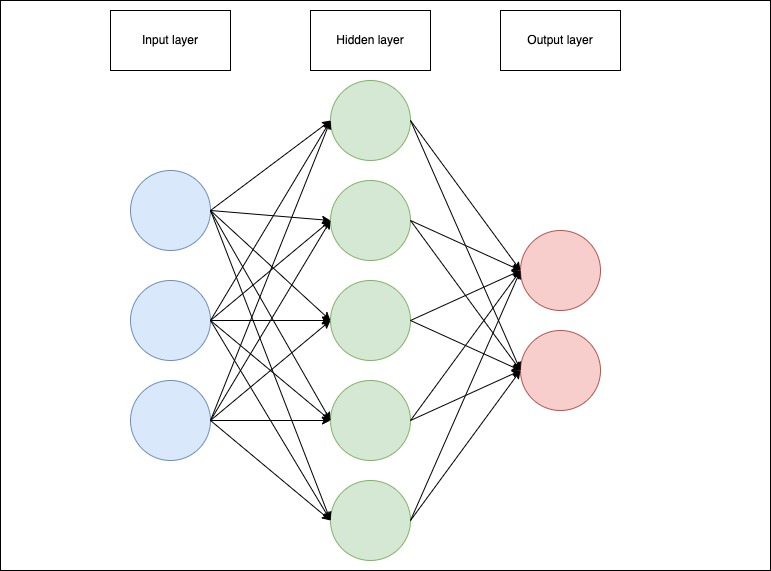
\includegraphics[width=\linewidth]{Figures/Machinelearning/nn_diagram.jpeg}
    \caption[Simple diagram of a neural network]{Simple neural network diagram drawm using Draw.io. Here the blue dots are the input layer, the green dots are a hidden layer, 
    and the red dots are the output layer. The arrows shows the connections between the nodes. }
    \label{fig:nndiagram}
\end{figure}

In order to avoid confusion, we will adhere to table \ref{tab:notation} for the notation used in the following sections.

% Define new columns types 
\newcolumntype{L}[1]{>{\raggedright\arraybackslash}p{#1}} % left fixed width
\newcolumntype{C}[1]{>{\centering\arraybackslash}p{#1}} % center fixed width
\newcolumntype{R}[1]{>{\raggedleft\arraybackslash}p{#1}} % flush right fixed width
\begin{table}
    % \setlength{\tabcolsep}{15pt}
    \renewcommand{\arraystretch}{1.3}
    \begin{center}
    \caption{Notation}
    \begin{tabular}{|C{1.5cm}|L{4cm}|C{2cm}|} \hline
    \multicolumn{3}{|c|}{Matrices and vectors}  \\ \hline
    Notation & \multicolumn{1}{c|}{Description} & Type \\ \hline
    $X$ & Design Matrix (input data). & $\mathbb{R}^{N\times \text{\#features}}$ \\ \hline
    $t$ & Target values. & $\mathbb{R}^{N\times \text{\#categories}}$ \\ \hline
    $y$ & Model output, the prediction from our network. &  $\mathbb{R}^{N\times \text{\#categories}}$\\ \hline
    $W^l$ & The weight matrix associated with layer $l$ which handles the connections between layer $l-1$ and $l$ . & $\mathbb{R}^{n_{l-1} \times n_l}$ \\ \hline
     $B^l$ & The bias vector associated with layer $l$ which handles the biases for all nodes in layer $l$.  & $\mathbb{R}^{n_{l} \times 1}$ \\ \hline
   
    \multicolumn{3}{|c|}{Elements}  \\ \hline
    $w^l_{ij}$ & The weight connecting node $i$ in layer $l-1$ to node $j$ in layer $l$. & $\mathbb{R}$ \\ \hline
    $b^l_j$ & Bias acting on node $j$ in layer $l$.  & $\mathbb{R}$ \\ \hline
    $z^l_j$ & Node output before activation on node $j$ on layer $l$. & $\mathbb{R}$\\ \hline
    $a^l_j$ & Activated node output on node $j$ on layer $l$. & $\mathbb{R}$ \\ \hline
    \multicolumn{3}{|c|}{Functions}  \\ \hline
    $C$ & \multicolumn{2}{l|}{Cost function} \\ \hline
    $\sigma^l$ & \multicolumn{2}{l|}{Activation function associated with layer $l$.} \\ \hline
    \multicolumn{3}{|c|}{Quantities }  \\ \hline
    $n_l$ & \multicolumn{2}{l|}{The number of nodes in layer $l$.} \\ \hline
    $L$ & \multicolumn{2}{l|}{Number of layers in total with $L-2$ hidden layers.} \\ \hline
    $N$ & \multicolumn{2}{l|}{Total number of data points.} \\ \hline
    \multicolumn{3}{|l|}{All indexing starts from 1: $i,j,k,l = 1, 2, \hdots$}  \\ \hline
    \end{tabular}
    \label{tab:notation}
    \caption{Table containing notation used for deriving the mathematical formulas for the neural network \cite{FYSSTK}}
  \end{center}
\end{table}
   

\subsection*{Gradient descent}
Let us now consider a general n-dimensional problem, with parameters $\boldsymbol{\theta} = \{\theta_1, \theta_2, ..., \theta_n\}$. 
Our objective is to find the set of $\boldsymbol{\theta}$ to minimize a cost function with respect to the data and target. 
One way to solve this problem is using ordinary least squares. For this approach, 
the optimal paramters $\boldsymbol{\theta_{opt}}$ are derived from minimizing the cost function, as shown here:
\begin{equation*}
    \boldsymbol{\theta_{opt}} = (\boldsymbol{X}^T\boldsymbol{X})^{-1}\boldsymbol{X}^T\boldsymbol{t},
\end{equation*}
where $\boldsymbol{X}$ is the design matrix containing the data, and $\boldsymbol{t}$ is the target vector. This however leads to a problem. Suppose the design matrix is sufficiently large,
then the matrix inversion will get computaitonally expensive, or it might not even exist for a given $\boldsymbol{X}$. Thus, an alternative approch is to iteratively approximate the ideal 
parameters. \par 
Suppose we we have a cost function $C(\boldsymbol{\theta})$ for a given problem. We can approximate the minimum of the cost function by calculating
the gradient $\nabla_{\theta}C$ with respect to $\boldsymbol{\theta}$. The negative of this gradient indicates the direction for the minimum of $C$ when evaluating 
it in a specific point $\boldsymbol{\theta}_i$ in the parameter space \cite{FYSSTK}. This is formulized as follows 
\begin{equation}
    \boldsymbol{\theta}_{i+1} = \boldsymbol{\theta}_i - \eta\nabla_{\theta}C(\boldsymbol{\theta}_i),
\end{equation}
where $\eta$ is a step size, also called the learning rate. The choice of $\eta$ is not a trivial case. It is one of several 
hyperparameters\footnote{Give reference to hyperparameters}
that can be altered, and that highly depend on the given problem. With regards to the learning rate, there are only three situations to consider, shown in figure \ref{fig:lr_choice}.

\begin{figure}[H]
    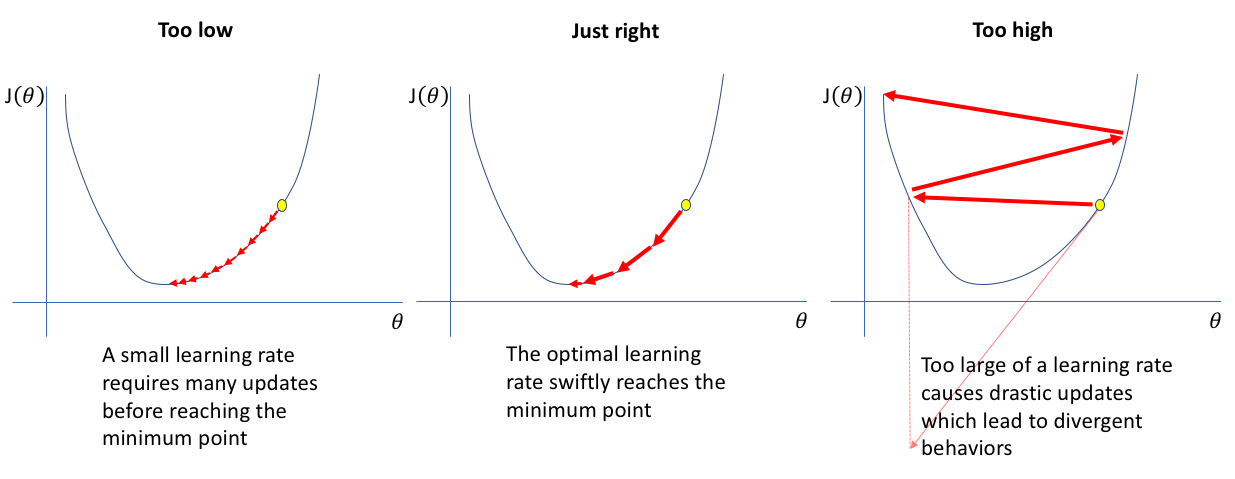
\includegraphics[width=\linewidth]{Figures/Machinelearning/lr_choice.png}
    \caption[Explaining concequence of choice of learning rate]{Figures showing different choices of learning rate for a given cost function, with respect to the tunable parameters. 
    Source: \href{https://www.jeremyjordan.me/content/images/2018/02/Screen-Shot-2018-02-24-at-11.47.09-AM.png}{Jeremy Jordan}, accessed 03.10.22.}
    \label{fig:lr_choice}
\end{figure}

Figure \ref{fig:lr_choice} visualizes the relation between the learning rate and the cost function. In the left most figure we note that the learning rate is too small. 
This leads to many iterations before you reach a minimum. In the right most figure we note that the learning rate is too high, and the result is that we get divergent behavior. 
Thus the goal is to find the optimal learning rate, shown in the middle figure. \par 
A modified and prefered version of gradient descent is the so called stochastic gradient descent. Regular gradient descent can, for large datasets be quite slow, and is prone to 
getting stuck in a local minima. To circumvent this issue, mini batches are introduced. 




\subsection*{Feed forwarding}
Inference (prediction) and training both use the same feed-forward algorithm. Lets then assume that we have generated a network. The network initializes the weights and biases usually 
with normal or uniformly distributed values, that can later be tuned. The procedure is to send the data through the network, weighting each connection according to the networks architecture,
and produce an output. The procedure can be summarized in the following steps \cite{FYSSTK}:
 \begin{itemize}
    \item The data is recieved by the input nodes in the network for each feature.
    \item Each input node weights the data value according to the connection of each node in the next layer.
    \item Every node in the hidden layers sums the weighted data values, and adds the bias associated to the given node, denoted as z. 
    \item This value z is then sent through an activation function $\sigma$, which produces the output of the node, denoted as $a = \sigma(z)$.
    \item This process is repeated for each hidden layer, and it is important to note that the number of nodes in the hidden layers is not dependent on the number of features in the original dataset. 
    \item The last hidden layer then sends the activated values to the output layer, where the number of nodes and choice of activation function depends on the problem to solve.
 \end{itemize}

Mathematically this is expressed as follows:
\begin{equation}
    z_j^l = \sum_{i=1}^{n_{l-1}} w_{ij}^l a_i^{l-1} + b_j^l, \quad a_j^l = \sigma^l(z_j^l),
\end{equation}
where $l$ is the layer index, $j$ is the node index, and $i$ is the index of the node in the previous layer, and $l \neq 1$, as it is not used on the input layer.


\subsection*{Backpropagation}
The way neural networks learn is conventionally by the use of the backpropagation algorithm, first proposed by Rumelhart et al\cite{backprop}. This is a bit misleading, 
as the backpropagation algorithm actually only refers to how to compute the gradient\cite{Goodfellow-et-al-2016}. The algorithm allows us to alter the weights and biases such that
we get an ideal output. Assuming a cost function $C$, we can calculate the gradient $\nabla_{w, b}C$, and use this to back propagate the error correction. The gradient $\nabla_{w, b}C$ is comprised of 
two derivatives
\footnote{NOTE TO SELF:: Note that this calculation is not a generalized algorithm for backpropagation, but rather for a special case using MSE.}\par
:\par 

\begin{equation*}
    \nabla_{w, b}C = \left(\frac{\partial C}{\partial w_{i,j}^l}, \frac{\partial C}{\partial b_j^l}\right).
\end{equation*}

We have to use the chain rule to calculate the derivatives, and using that the last layer is $l=L$, we get the derivative with respect to the weights as 

\begin{equation*}
    \frac{\partial C}{\partial w_{i,j}^L} = \frac{\partial C}{\partial a_j^L}\frac{\partial a_j^L}{\partial z_j^L}\frac{\partial z_j^L}{\partial w_{i,j}^L},
\end{equation*}
where 
\begin{equation*}
    a_j^L = \sigma(z_j^L), \quad z_j^L = \sum_{i=1}^{n_L-1} w_{i,j}^La_i^{L-1} + b_j^L.
\end{equation*}

This then gives us 
\begin{equation*}
    \frac{\partial C}{\partial w_{i,j}^L} = \frac{\partial C}{\partial a_j^L}\sigma'(z_j^L)a_i^{L-1},
\end{equation*}
where we defined that 
\begin{equation}\label{eq:sigma_der}
    \sigma'(z_j^L) = \frac{\partial a_j^L}{\partial z_j^L}.
\end{equation}

This derivative is very easy to calculate given a specific cost function and activation function. The derivative with respect to the bias is given as follows:

\begin{equation*}
    \frac{\partial C}{\partial b_k^L} = \frac{\partial C}{\partial a_j^L}\frac{\partial a_j^L}{\partial z_j^L}\frac{\partial z_j^L}{\partial b_{j}^L},
\end{equation*}
which gives us the final expression as 

\begin{equation*}
    \frac{\partial C}{\partial b_k^L} = \frac{\partial C}{\partial a_j^L}\sigma'(z_j^L). 
\end{equation*}

We will now introduce a new notation, a local gradient commonly called the "error". It reflects how the rate of change of the cost function depends on the j'th node in the l'th layer.

\begin{equation*}
    \delta_j^l \equiv \frac{\partial C}{\partial z_j^l}.  
\end{equation*}
Using this we get the following expression:

\begin{equation*}
    \delta_j^L=  \frac{\partial C}{\partial z_j^L} = \frac{\partial C}{\partial a_j^L}\frac{\partial a_j^L}{\partial z_j^L} = \frac{\partial C}{\partial a_j^L}\sigma'(z_j^L),
\end{equation*}

giving us the more compact forms of the derivatives with respect to the weights and biases:

\begin{equation*}
    \frac{\partial C}{\partial w_{i,j}^L} = \delta_j^La_i^{L-1}, \quad \frac{\partial C}{\partial b_j^L} = \delta_j^L.
\end{equation*}

We can now let $\boldsymbol{\delta^l}$ be the vector of all the errors in the l'th layer, and $\boldsymbol{\delta^L}$ be the vector of all the errors in the last layer. 
The error in the l'th layer can then be expressed as a matrix equation for the last layer as follows:

\begin{equation*}
    \boldsymbol{\delta^l} = \nabla_aC \odot \frac{\partial \sigma}{\partial z^L}, \quad \nabla_aC = \left[\frac{\partial C}{\partial a_1^L}, \frac{\partial C}{\partial a_2^L}, ..., \frac{\partial C}{\partial a_{n_L}^L} \right]^T.
\end{equation*}

Here $\odot$ is the Hadamard product (element wise product). This local gradient can now be defined recursively for the j'th node in a layer l as a function of the local error in the next layer:

\begin{equation}
    \label{eq:localgradient}
    \delta_j^l \equiv \frac{\partial C}{\partial z_j^l} = \sum_k \frac{\partial C}{\partial z_k^{l+1}}\frac{\partial z_k^{l+1}}{\partial z_j^l} = \sum_k \frac{\partial z_k^{l+1}}{\partial z_j^l} \delta_k^{l+1}.
\end{equation}

We also note that 
\begin{equation*}
    z_k^{l+1} = \sum_{j=1}^{n_l} w_{j,k}^{l+1}a_j^l + b_k^{l+1} = \sum_{j=1}^{n_l} w_{j,k}^{l+1}\sigma(z_j^l) + b_k^{l+1},
\end{equation*} 
thus the partial derivative is given as 

\begin{equation}
    \label{eq:dzl1dz}
    \frac{\partial z_k^{l+1}}{\partial z_j^l} = w_{j,k}^{l+1}\sigma'(z_j^l), 
\end{equation}
using the substitution from equation \ref{eq:sigma_der}. This allows us to substitute equation \ref{eq:dzl1dz} into equation \ref{eq:localgradient} to get the following expression:

\begin{equation}
    \label{eq:localgradient2}
    \delta_j^l = \sum_k w_{j,k}^{l+1}\sigma'(z_j^l)\delta_k^{l+1}.
\end{equation}

Using this we can derive a three step formula for the backpropagation algorithm:
\begin{itemize}
    \item Compute the local gradient for the last layer, $\delta^L$.
    \item Recursively compute the local gradient for the remaining layers, $\delta^l$ for $l=L-1, L-2, ..., 1$.
    \item Update the weights and biases for all layers, $l=1, 2, ..., L$, given the learning rate $\eta$ as shown below: 
\end{itemize}

\begin{equation*}
    w_{i,j}^{l} \leftarrow w_{i,j}^{l} - \eta \delta_j^l a_i^{l-1},
\end{equation*}


\begin{equation*}
    b_j^l \leftarrow b_j^l - \eta \delta_j^l.
\end{equation*}
